\chapter{Task 44 - Social Connectedness Index II from Facebook}
\label{ch:task44}

\section{Theoretical Introduction}

This analysis investigates how geographical distance, administrative boundaries, and socio-economic factors structurally shape online communities through the lens of spatial network theory. The empirical characterization of these sub-national social networks is conducted utilizing the \textbf{Meta Social Connectedness Index (SCI) II} database, which measures the relative friendship probability between administrative locations $i$ and $j$ defined as:\cite{bailey2018social}

\begin{equation}\label{eq:sci_definition}
    SCI_{i,j}=\frac{\text{Friendships}_{i,j}}{\text{Pop}_i \times \text{Pop}_j}
\end{equation}

where $\text{Friendships}_{i,j}$ represents the total number of Facebook links between the two regions, and $\text{Pop}_i, \text{Pop}_j$ reflect the respective cohorts of active users.\cite{bailey2018social} By filtering out cross-border connections, this work inspects administrative fragmentation, spatial mixing via a distance-decay framework, and national structural regimes—ranging from centralized hubs to polycentric topologies—based on network size and strength heterogeneity metrics.

\section{Dataset and Network Construction}
The pipeline retains exclusively within-country edges, filtering the top $100$ nations by sub-national region count.\cite{hdx2026facebook} The United States ($US$) are excluded to avoid macro-scaling distortions. The target countries are split into two layers based on data availability: European territories mapped to the \textbf{NUTS3} framework and non-European territories mapped to \textbf{GADM Level 1}.

Shapefiles are downloaded from GADM for the non-European layer,\cite{gadm2025database} and the NUTS 2024 GeoJSON is gathered from Eurostat.\cite{eurostat2024nuts} Spatial coordinates are computed as the representative points of the regional geometries. Symmetric duplicates are averaged into undirected edges, and self-loops are omitted. The final parsed network integrates both layers, yielding $N = 3,147$ nodes and $E = 136,844$ edges.

The distribution of regions per country shows a severe fragmentation asymmetry captured by a lognormal PDF fit: most nations have fewer than $30$ subdivisions, while a few exceed $100$. Germany ($DEU$) is the main outlier with $399$ nodes due to its granular NUTS3 framework.

\begin{figure}[htbp]
    \centering
    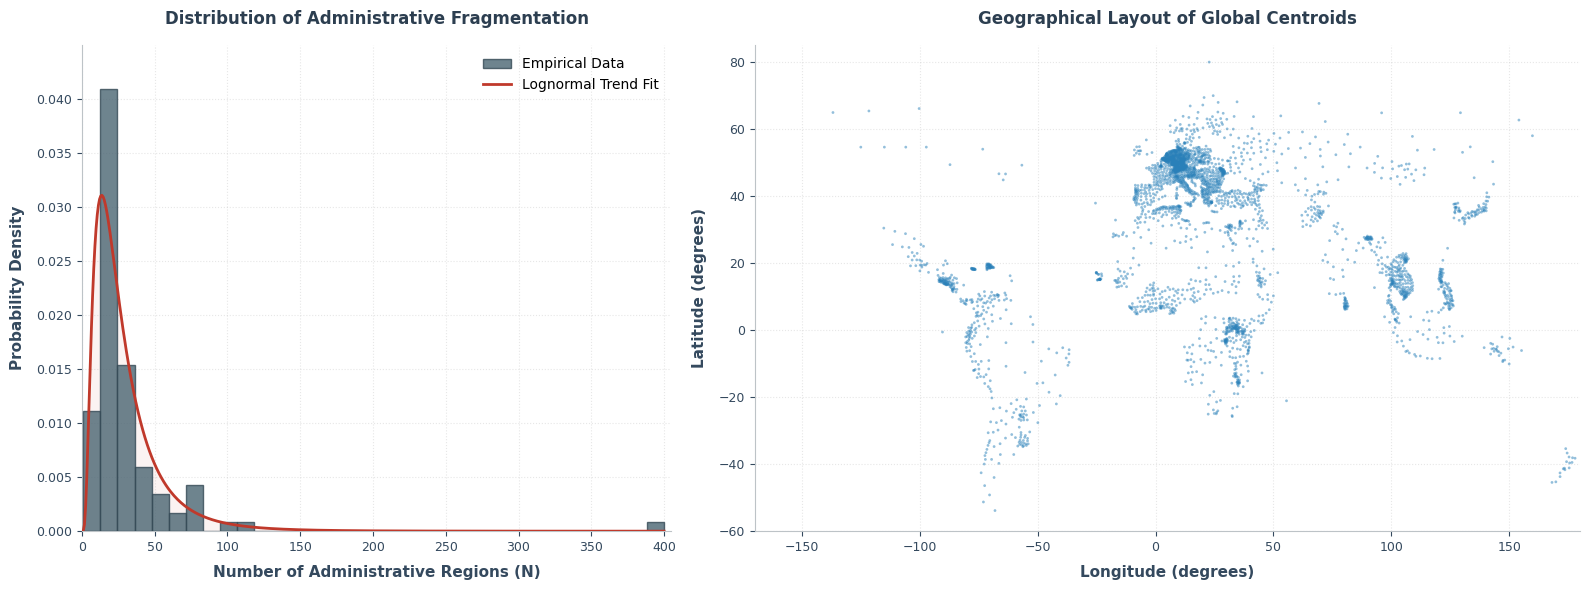
\includegraphics[width=0.95\textwidth]{images/1_preliminary_characterization.png}
    \caption{(Left) Distribution of administrative fragmentation ($N$) fitted with a Lognormal PDF trend. (Right) Geographical layout of global regional centroids computed from shapefile geometries.}
    \label{fig:preliminary_characterization}
\end{figure}

\section{Network Data Analytics}

A quadratic scaling law links the number of edges to the network size ($E \sim N^{2.03}$, $R^2 = 1.00$), meaning the networks are topologically complete cliques with an unweighted density $\rho = 1$. The real degrees of freedom are stored within the link intensities. The probability density of $\log_{10}(SCI)$ is heavily right-skewed and spans six orders of magnitude, separating a dense backbone of weak interactions from a narrow tail of intense regional flows.

\begin{figure}[htbp]
    \centering
    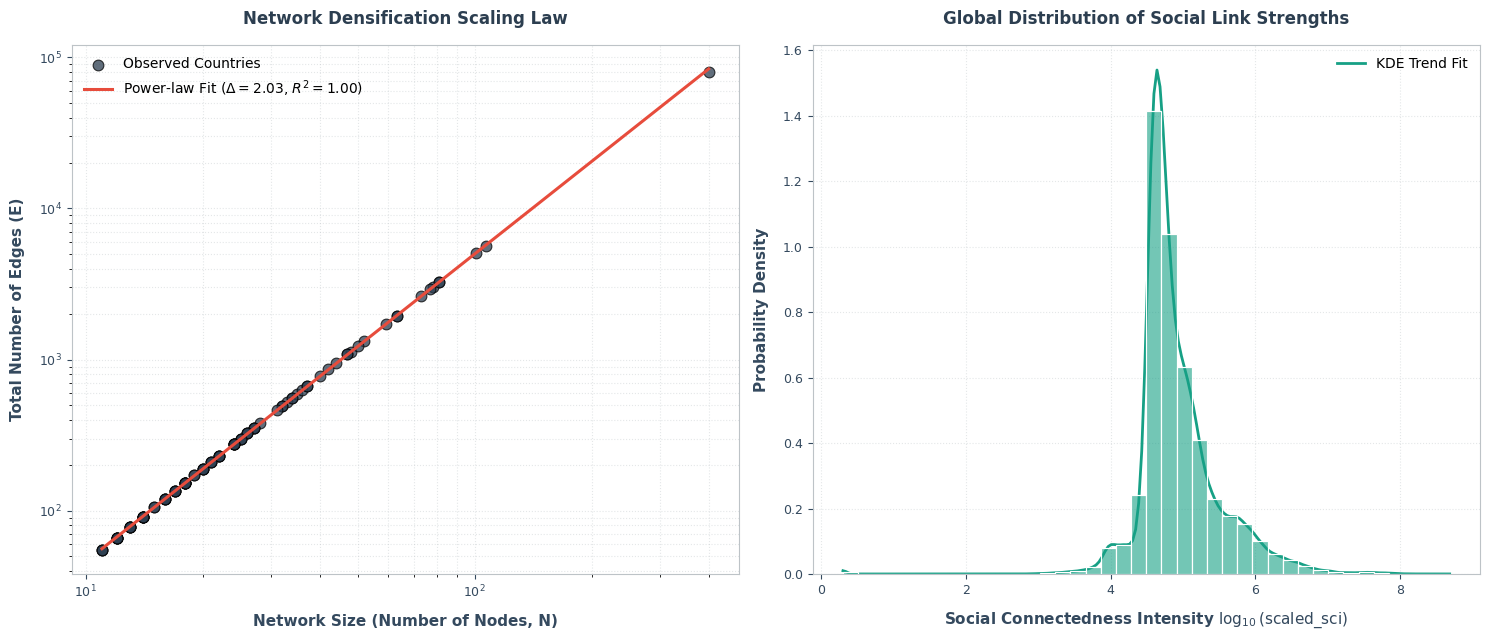
\includegraphics[width=0.95\textwidth]{images/5_network_general_characterization.png}
    \caption{(Left) Network densification scaling law mapping $N$ vs $E$ in log-log scale. (Right) Global probability density distribution of the social link weights.}
    \label{fig:network_scaling_and_weights}
\end{figure}

Integrating geospatial coordinates, we fit the link intensities to a power-law distance-decay Gravity Law using Haversine distance: $SCI_{ij} \sim d_{ij}^{-\alpha}$. The linear fit yields a global exponent $\alpha=0.78$, demonstrating that virtual connections decrease almost inversely with distance. The highest density of connections is packed within the $100$--$600$~km range, while long-range tails extend beyond $10,000$~km.

Network organization is summarized via the Gini coefficient ($G\in[0,1]$) on node strengths $\{s_i\}$.\cite{hu2011gini} Mapping countries into a phase space defined by size and heterogeneity relative to their global medians yields four structural regimes: \textit{Small and Concentrated}, \textit{Large and Concentrated}, \textit{Small and Homogeneous}, and \textit{Large and Homogeneous}. The upper right quadrant represents centralized topologies with a dominant hub, like Colombia ($COL$, $G > 0.30$). The bottom right represents fragmented yet uniform networks, like Japan ($JPN$, $G \approx 0.07$). The bottom left quadrant accommodates small, homogeneous networks like Jamaica ($JAM$).

\begin{figure}[htbp]
    \centering
    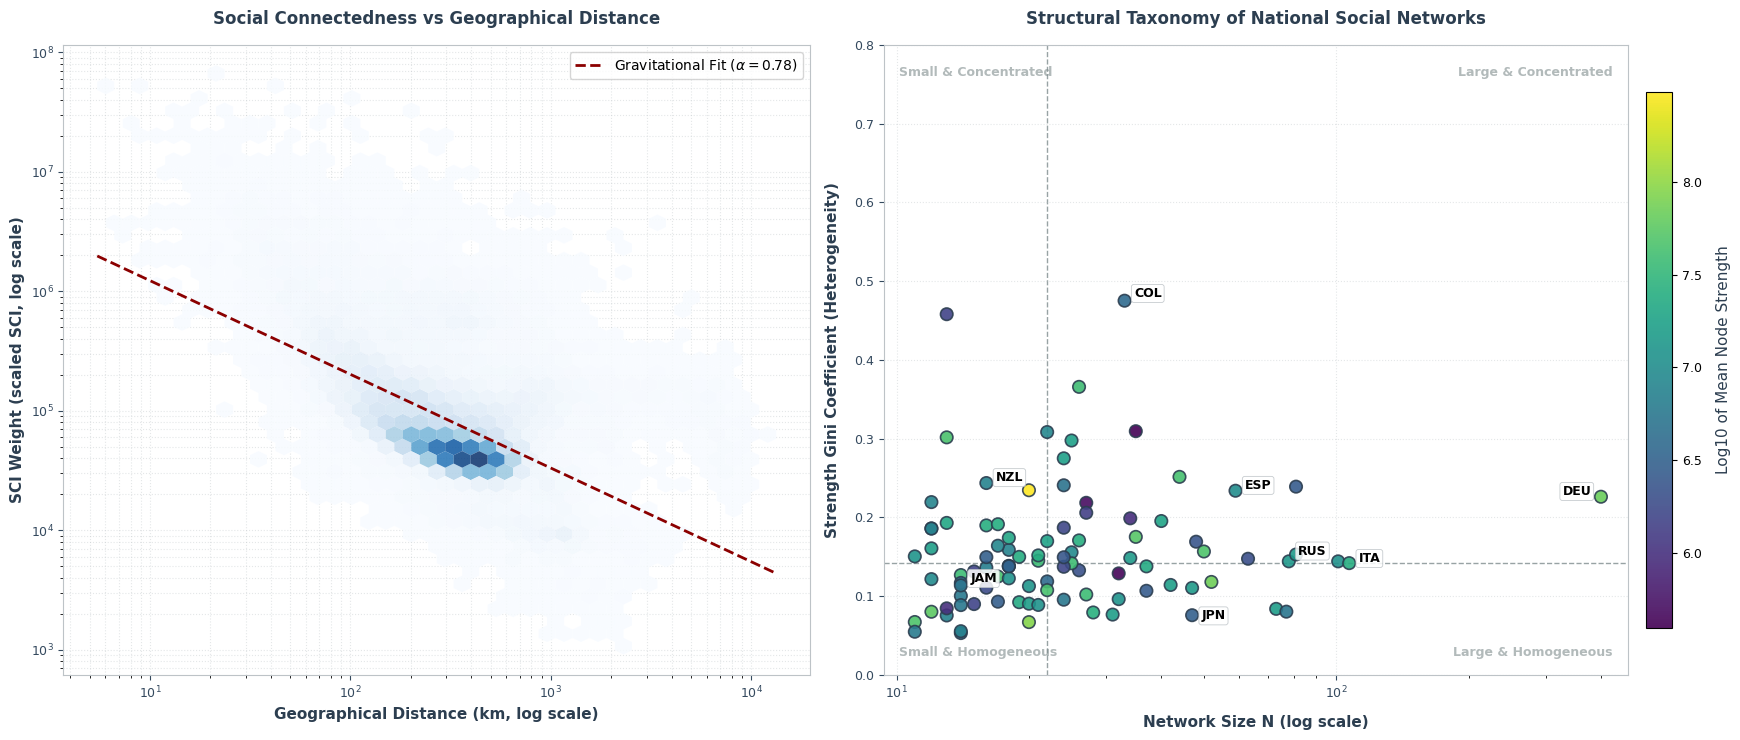
\includegraphics[width=0.95\textwidth]{images/combined_analysis_and_taxonomy.png}
    \caption{(Left) Empirical scaling of SCI weight as a function of Haversine geographical distance fitted via log-log linear regression. (Right) Structural taxonomy phase space of national social networks based on size $N$ and strength Gini coefficient.}
    \label{fig:combined_analysis_taxonomy}
\end{figure}

Italy occupies a borderline position exactly on the global Gini median line ($G \approx 0.14$). The economic dominance of major centers (Milan, Rome) acts as a centripetal force pulling the Gini upward. However, this concentration is mitigated by a decentralized, polycentric regional structure with strong secondary nodes and interconnected clusters. This polycentric equilibrium anchors the Italian macro-social network in a stable transition state between homogeneity and centralization.